\documentclass{beamer}


\usepackage{alltt}
\usepackage{tikz}
\usepackage{tikz-qtree}

\usepackage{color}
\newcommand{\red}[1]{{\color{red}#1}}
\newcommand{\cyan}[1]{{\color{cyan}#1}}
\newcommand{\blue}[1]{{\color{blue}#1}}
\newcommand{\magenta}[1]{{\color{magenta}#1}}
\newcommand{\yellow}[1]{{\color{yellow}#1}}
\newcommand{\green}[1]{{\color{green}#1}}

\newcommand{\sect}[1]{
\section{#1}
\begin{frame}[fragile]\frametitle{#1}
}

\newcommand{\bi}{\begin{itemize}}
\newcommand{\ii}{\item}
\newcommand{\ei}{\end{itemize}}


\title
{
Scheme Notes 01
}

\subtitle{
} % (optional)

\author[Geoffrey Matthews]
{Geoffrey Matthews}
% - Use the \inst{?} command only if the authors have different
%   affiliation.

\institute[WWU/CS]
{
  Department of Computer Science\\
  Western Washington University
}
\begin{document}
\begin{frame}
\titlepage
\end{frame}



\sect{Resources}
\bi
\ii The software:
\bi\ii \url{https://racket-lang.org/}\ei
\ii Texts:
\bi
\ii \url{https://mitpress.mit.edu/sicp/}
\ii \url{http://www.scheme.com/tspl3/}\\ (make sure you use the 3rd
edition and not the 4th)
\ii \url{http://ds26gte.github.io/tyscheme/}
\ei
\ei
\end{frame}


\sect{Running the textbook examples}

\bi
\ii Using the racket language is usually best, the examples from
    {\em The Scheme Programming Language} should run without modification.

 \ii The examples from SICP are a little more idiosyncratic.  Most of
 them can be run by installing the {\tt sicp} package as in
 these instructions:\\
 \url{http://stackoverflow.com/questions/19546115/which-lang-packet-is-proper-for-sicp-in-dr-racket}

 \ei
\end{frame}

\sect{Every powerful language has}


\bi
\ii primitive expressions: the simplest entities, such as \verb|3| and \verb|+|
\ii
means of combination: buidling compound elements from simpler ones such as 

\verb|(+ 3 4)|
\bi
\ii In Scheme combinations are always parentheses, with the operator
first and the operands following.
\ei
\ii
means of abstraction: a way for naming compound elements and then manipulating them as units such as 

\verb|(define pi 3.14159)|

\verb|(define square (lambda (x) (* x x)))|
\ei

\end{frame}

\sect{The REPL does the following three things:}

\bi
\ii Reads an expression
\ii Evaluates it to produce a value
\ii Prints the value
\ei

The returned value has a small set of types, including number, boolean and procedure. (Later, we'll see symbol, pair, vector, and promise (stream).)

\end{frame}



\sect{There are 4 types of expressions:}
\bi
\ii Constants: numbers, booleans. Examples: \verb|4 3.141592 #t #f|
\ii Variables: names for values. We create these using the special form \verb|define|
\ii Special forms: have special rules for evaluation. In addition, you may not redefine a special form.
\ii Combinations: \verb|(<operator> <operands>)|. These are sometimes called "function calls" or "procedure applications."
\ei 

The first two types of expressions (constants and variables) are
primitive expressions -- they have no parentheses. The second two
types are called compound expressions -- they have parentheses.

\end{frame}

\sect{Mantras}
\bi
\ii Every expression has a value
\bi\ii(except for errors, infinite loops and the 
\verb|define| special form)\ei
\ii To find the value of a combination:
\bi
\ii Find values of all subexpressions in any order
\ii Apply the value of the first to the values of the rest
\ei
\ii The value of a \verb|lambda| expression is a procedure
\ei
\end{frame}

\sect{Finding the value of a combination}
\bi
\ii Find values of all subexpressions in any order
\ii Apply the value of the first to the values of the rest
\begin{alltt}
    (+ (* 2 3) \fbox{(- 8 2)})

    (+ \fbox{(* 2 3)}    6   )

   \fbox{(+    6       6   )}

            12
\end{alltt}
\ei
\end{frame}













\sect{\large Program Evaluation In Lisp}

A process of {\em tree accumulation.}
\begin{alltt}
(* (+ 2 (* 4 6))
   (+ 3 5 7))
\end{alltt}

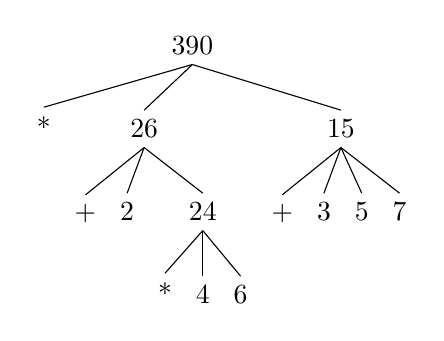
\begin{tikzpicture}
  \Tree
      [.390
        [.* ]
        [.26
          [.+ ]
          [.2 ]
          [.24
            [.* ]
            [.4 ]
            [.6 ]
          ]
        ]
        [.15
          [.+ ]
          [.3 ]
          [.5 ]
          [.7 ]
        ]
      ]
\end{tikzpicture}




\end{frame}
\sect{Introducing Local Variables}

\begin{alltt}
(let ((x 3)
      (y 4)
      (z 5))
    (+ x (* y z)))   =>  23
\end{alltt}


\end{frame}
\sect{Beware!  This will NOT work.}

\begin{alltt}
(let ((x 3)
      (y (* 2 x))
      (z (* 3 x)))
    (+ x (* y z)))   =>  57
\end{alltt}


\end{frame}
\sect{But this will.}

\begin{alltt}
(\red{let*} ((x 3)
       (y (* 2 x))
       (z (* 3 x)))
    (+ x (* y z)))   =>  57
\end{alltt}


\end{frame}
\sect{Defining Procedures}

Two equivalent ways:
\begin{alltt}
(define \red{(square x)} (* x x))
(define square (lambda (x) (* x x)))
\end{alltt}
The first one is more in line with the procedure call:
\begin{alltt}
\red{(square 5)} => 25
\end{alltt}

\end{frame}
\sect{Defining Procedures}

Two equivalent ways:
\begin{alltt}
(define (square x) (* x x))
(define square \red{(lambda (x) (* x x))})
\end{alltt}
The second one is more in line with defining other things:
\begin{alltt}
(define x \red{(* 3 4)})
(define y \red{(list 'a 'b 'c)})
\end{alltt}
The action of {\tt define} is simply to give a {\sl name} to
the result of an expression.

\end{frame}
\sect{Defining Procedures}

Two equivalent ways:
\begin{alltt}
(define (square x) (* x x))
(define square \red{(lambda (x) (* x x))})
\end{alltt}
The result of a lambda-expression is an anonymous function.
\\
We can name it, as above, or use it without any name at all:
\begin{alltt}
(square 5) => 25
(\red{(lambda (x) (* x x))} 5) => 25
\end{alltt}

\end{frame}
\sect{Solving problems}
{\small
Newton's method: \\
If $y$ is a guess for $\sqrt{x}$, then 
the average of $y$ and $x/y$ is an even better guess.

\begin{tabular}{cccc}
$x$ & guess & quotient & average\\
2 & 1.0 & 2.0 & 1.5\\
2 & 1.5 & 1.3333333333333333 & 1.4166666666666665\\
2 & 1.4166666666666665 & 1.411764705882353 & 1.4142156862745097\\
2 & 1.4142156862745097 & 1.41421143847487 & 1.4142135623746899\\
...
\end{tabular}
Evidently, we want to iterate, and keep recomputing
these things until we find a value that's close enough.
}

\end{frame}
\sect{Newton's Method in Scheme}
{\scriptsize
\begin{verbatim}
(define sqrt-iter 
  (lambda (guess x)
    (if (good-enough? guess x)
        guess
        (sqrt-iter (improve guess x) x))))

(define improve 
  (lambda (guess x)
    (average guess (/ x guess))))

(define average 
  (lambda (x y) (/ (+ x y) 2)))

(define good-enough? 
  (lambda (guess x)
    (< (abs (- (square guess) x)) 0.00001)))

(define square 
  (lambda (x) (* x x)))

(define sqrt 
  (lambda (x) (sqrt-iter 1.0 x)))
\end{verbatim}
}
Decompose big problems into smaller problems.

\end{frame}
\sect{Definitions can be nested}
\begin{alltt}
(define sqrt 
  (lambda (x)
\blue{    (define good-enough? 
      (lambda (guess x)
        (< (abs (- (square guess) x)) 0.001)))
    (define improve 
      (lambda (guess x)
        (average guess (/ x guess))))
    (define sqrt-iter 
      (lambda (guess x)
        (if (good-enough? guess x)
            guess
            (sqrt-iter (improve guess x) x))))}
    (sqrt-iter 1.0 x)))
\end{alltt}

\end{frame}
\sect{Parameters need not be repeated}
\begin{alltt}
(define sqrt 
  (lambda (\blue{x})
    (define good-enough? 
      (lambda (\red{guess})
        (< (abs (- (square \red{guess}) \blue{x})) 0.001)))
    (define improve 
      (lambda (\red{guess})
        (average \red{guess} (/ \blue{x} \red{guess}))))
    (define sqrt-iter 
      (lambda (\red{guess})
        (if (good-enough? \red{guess})
            \red{guess}
            (sqrt-iter (improve \red{guess})))))
    (sqrt-iter 1.0)))
\end{alltt}
\end{frame}
\sect{Introducing local functions with {\tt letrec} }
\begin{alltt}
(define sqrt 
  (lambda (x)
    (letrec ((good-enough? 
              (lambda (guess)
                (< (abs (- (square guess) x)) 0.001)))
             (improve 
              (lambda (guess)
                (average guess (/ x guess))))
             (sqrt-iter 
              (lambda (guess)
                (if (good-enough? guess)
                    guess
                    (sqrt-iter (improve guess)))))
             )
             (sqrt-iter 1.0))))
\end{alltt}

\end{frame}
\sect{Procedures as parameters}

Summation notation: \[\sum_{i=a}^{b} f(i) = f(a) + \ldots + f(b)\]

In scheme:
\begin{alltt}
(define sum
  (lambda (a b \blue{f})
    (if (> a b)
        0
        (+ (\blue{f} a) (sum (+ a 1) b \blue{f})))))

(sum 1 10 \blue{square}) => 385
(sum 1 10 \blue{(lambda (x) (* x x x))}) => 3025
\end{alltt}

\end{frame}
\sect{Finding fixed points}

$x$ is a {\sl fixed point} of $f$ if $x = f(x)$

For some functions you can find fixed points by iterating:
\\
$x, f(x), f(f(x)), f(f(f(x))), \ldots$

\end{frame}
\sect{Fixed points in scheme:}
{\scriptsize
\begin{alltt}
(define fixed-point
  (lambda (f)
    (let 
        ((tolerance 0.0001)
         (max-iterations 10000))
      (letrec 
          ((close-enough? 
            (lambda (a b) (< (abs (- a b)) tolerance)))
           (try 
            (lambda (guess iterations)
              (let ((next (f guess)))
                (cond ((close-enough? guess next) next)
                      ((> iterations max-iterations) #f)
                      (else (try next (+ iterations 1)))))))
           )
        (try 1.0 0)))))

(fixed-point cos)  => 0.7390547907469174
(fixed-point sin)  => 0.08420937654137994
(fixed-point (lambda (x) x)) => 1.0
(fixed-point (lambda (x) (+ x 1))) => #f
\end{alltt}
}

\end{frame}
\sect{Remember Newton's Method?}

\begin{alltt}
(define sqrt
  (lambda (x)
    (fixed-point (lambda (y) (/ (+ y (/ x y)) 2)))))
\end{alltt}

\end{frame}
\sect{Procedures as Returned Values}
\begin{alltt}
(define make-adder
  (lambda (n)
    (lambda (m) (+ m n))))
\end{alltt}
\end{frame}
\sect{Procedures as Returned Values}

\begin{alltt}
(define average-damp 
  (lambda (f)
    (lambda (x) (/ (+ x (f x)) 2))))

(define sqrt
  (lambda (x)
    (fixed-point (average-damp (lambda (y) (/ x y))))))
\end{alltt}


\end{frame}
\end{document}
